\chapter{Marco teórico}

\section{Inteligencia artificial, aprendizaje automático y aprendizaje profundo}

Delimitemos en primer lugar el significado de las diferentes disciplinas que la ingeniería utiliza a la hora de estudiar y desarrollar sistemas de inteligencia artificial. Es frecuente encontrar que términos como \textit{inteligencia artificial} (\textit{Artificial Inteligence}), \textit{aprendizaje automático} (\textit{Machine Learning}) y \textit{aprendizaje profundo} (\textit{Deep Learning}) se utilizan de manera indistinta. Sin embargo, cada uno de ellos tiene un significado específico y es importante distinguirlos para comprender el estado actual de la investigación en el área. Sin embargo, estos conceptos se entienden de forma jerárquica \cite{}, donde la inteligencia artificial es el concepto más amplio, que incluye al \textit{aprendizaje automático} y este a su vez al \textit{aprendizaje profundo}.

\begin{figure}[H]
    \centering
    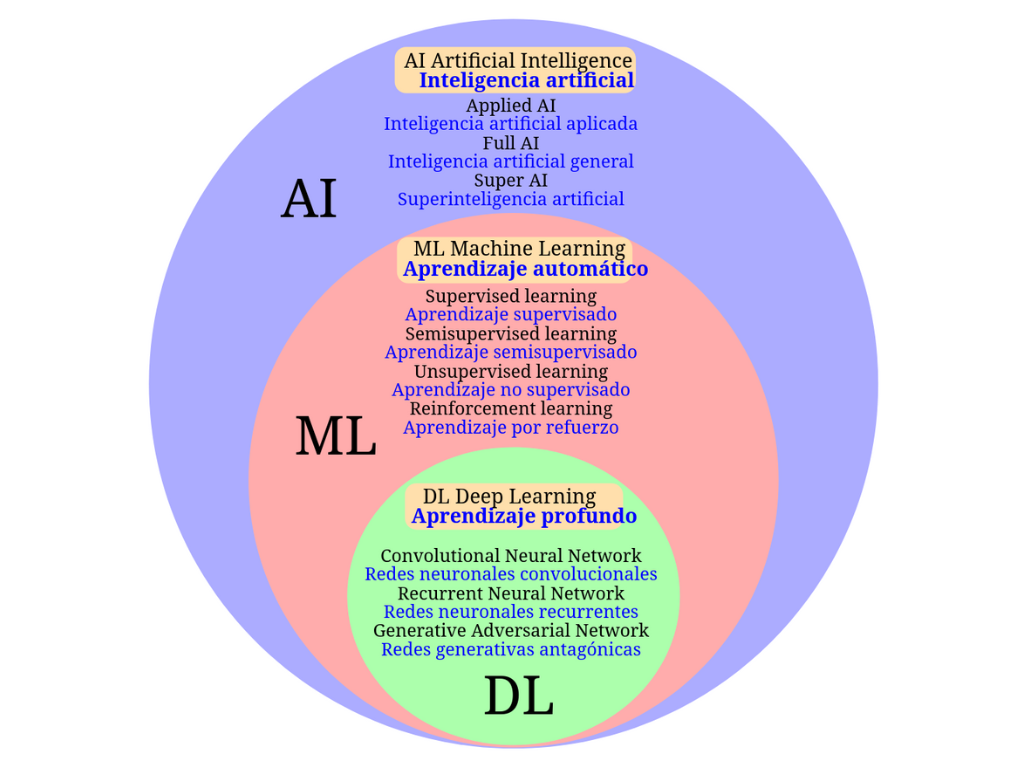
\includegraphics[width=0.8\textwidth]{./figuras/Tipos_Inteligencia_Artificial.png}
    \caption[Tipos de Inteligencia Artificial]{Tipos de Inteligencia Artificial, adaptado por Jzh2074 basado en Wang et al. (2021). Fuente: Jzh2074 \protect\citeyear{jzh2074}, Wikimedia Commons; Wang et al. \protect\citeyear{wang2021promising}.}
    \label{fig:ai_types}
\end{figure}


Tratemos de delimitar cada uno de estos conceptos.

\subsection{Inteligencia artificial}

La inteligencia artificial es el campo de estudio más antiguo de los tres, y no queda limitado al ámbito computacional. La inteligencia artificial ha sido objeto, en su sentido más amplio, por la filosofía. Los mismos racionalismos y estructuralismos, propios de los sistemas de pensamiento occidentales, están en la base conceptual de la inteligencia artificial. No será, no obstante, hasta el siglo XX donde se comience a plantear de forma explícita la posibilidad matemática de un sistema capaz de generar inteligencia. En 1950, Alan Turing publica su artículo \textit{Computing Machinery and Intelligence} \cite{alan1950a}, donde propone un test para determinar si una máquina es capaz de pensar. Este test, conocido como \textit{Test de Turing}, en la interacción de una entidad humana con una artificial, a través de un terminal de texto como única interfaz. La máquina supera el test si el humano no es capaz de distinguir si la entidad con la que está interactuando es artificial o humana. A este test, a pesar de su escaso rigor y su restricción antropocéntrica del concepto de inteligencia, aún se apela de manera frecuente para valorar la capacidad de sistemas de IA modernos.

Sin embargo, el concepto de inteligencia artificial va más allá de la pura imitación humana, si bien no la excluye. Si tomamos la \emph{racionalidad} como un conjunto de estructuras lógicas, dentro de cuyos sistemas se engloba el pensamiento y racionalidad humanos, no es necesario que la inteligencia artificial se limite en su objetivo a superar el test de Turing. Las diferentes definiciones de inteligencia artificial que se han dado a lo largo de la historia han variado su acento según hayan puesto su mira en la imitación del pensamiento o acción \emph{humanos}, o en el pensamiento y acción \emph{racional} \cite{RussellStuartJ2021AI:A}.

Es a matemáticos como Turing o Curt Gödel a quienes debemos los fundamentos matemáticos de procesos de pensamiento como sistemas computacionales capaces de generar \textit{outputs} racionales a partir de \textit{inputs} arbitrarios. La idea de que el propio cerebro humano es una de las infinitas \emph{máquinas de Turing} posibles \cite{penroseNuevaMenteEmperador2015} ha sido un pensamiento muy atractivo y que ha impulsado la investigación de la IA computacional. Por otra parte, las investigaciones en \textit{procesamiento del lenguaje natural}, entre las que debemos de destacar el concepto de \emph{entropía} de Shannon \cite{shannon1951prediction}, que han ido parejas al desarrollo de los lenguajes de programación de computadoras, están en la base de los modernos sistemas de IA.

\subsection{Machine Learning}

El \textit{Machine Learning}, o \textit{aprendizaje automático} \dots


\section{Deep Learning}

qué es el Deep Learning, y por qué ha evolucionado tanto en los últimos años, factores: poder computacional, cantidad de datos disponibles, democratización de la computación, mejoras en las arquitecturas y modelos de Deep Learning.


\subsection{Tipos de redes neuronales}
\subsection{Datos y entrenamiento de modelos de \textit{Deep Learning}}
\subsection{La arquitectura Transformer}

\section{Modelos de lenguaje}

\subsection{Procesamiento del Lenguaje Natural}
\subsection{Grandes modelos de lenguaje}
\subsection{Modelos prentrenados}
\subsection{Ajuste fino de los modelos}

\section{Modelos de lenguaje y generación de código}
